%%%%%%%%%%%%%%%%%%%%%%%%%%%%%%%%%%%%%%%%%
% baposter Landscape Poster
% LaTeX Template
% Version 1.0 (11/06/13)
%
% baposter Class Created by:
% Brian Amberg (baposter@brian-amberg.de)
%
% This template has been downloaded from:
% http://www.LaTeXTemplates.com
%
% License:
% CC BY-NC-SA 3.0 (http://creativecommons.org/licenses/by-nc-sa/3.0/)
%
%%%%%%%%%%%%%%%%%%%%%%%%%%%%%%%%%%%%%%%%%

%----------------------------------------------------------------------------------------
%	PACKAGES AND OTHER DOCUMENT CONFIGURATIONS
%----------------------------------------------------------------------------------------

\documentclass[landscape,a0paper,fontscale=0.3]{baposter} % Adjust the font scale/size here

\usepackage{graphicx} % Required for including images
\graphicspath{{/home/alli/projects/talks/figures/}} % Directory in which figures are stored

\usepackage{amsmath} % For typesetting math
\usepackage{amssymb} % Adds new symbols to be used in math mode
\usepackage{booktabs} % Top and bottom rules for tables
\usepackage{enumitem} % Used to reduce itemize/enumerate spacing
\usepackage{palatino} % Use the Palatino font
\usepackage[font=small,labelfont=bf]{caption} % Required for specifying captions to tables and figures

\usepackage{multicol} % Required for multiple columns
\usepackage{subcaption}
\usepackage[firstinits=true,backend=bibtex,doi=false,isbn=false,url=false]{biblatex}
\AtEveryBibitem{%
  \clearfield{pages}%
}
\renewcommand{\bibfont}{\normalfont\scriptsize}
\addbibresource{/home/alli/common/refs.bib}

\defbibenvironment{bibliography}
  {\noindent}
  {\unspace}
  {\printtext[labelnumberwidth]{%
    \printfield{prefixnumber}%
    \printfield{labelnumber}}
    \addspace}
\renewbibmacro*{finentry}{\finentry\addspace}

\usepackage{setspace}
\setlength{\columnsep}{1.5em} % Slightly increase the space between columns
\setlength{\columnseprule}{0mm} % No horizontal rule between columns


\usepackage{tikz} % Required for flow chart
\usetikzlibrary{shapes,arrows} % Tikz libraries required for the flow chart in the template

\newcommand{\compresslist}{ % Define a command to reduce spacing within itemize/enumerate environments, this is used right after \begin{itemize} or \begin{enumerate}
\setlength{\itemsep}{1pt}
\setlength{\parskip}{0pt}
\setlength{\parsep}{0pt}
}

\definecolor{lightblue}{rgb}{0.145,0.6666,1} % Defines the color used for content box headers
\definecolor{darkpurple}{rgb}{0.28,0.24,0.55}

\newcommand{\Mod}[1]{\ (\mathrm{mod}\ #1)}



\begin{document}

\begin{poster}
{
headerborder=open, % Adds a border around the header of content boxes
colspacing=1em, % Column spacing
columns=3,
textfont=\Large,
bgColorOne=white, % Background color for the gradient on the left side of the poster
bgColorTwo=white, % Background color for the gradient on the right side of the poster
borderColor=darkgray, % Border color
headerColorOne=darkgray, % Background color for the header in the content boxes (left side)
headerColorTwo=darkpurple, % Background color for the header in the content boxes (right side)
headerFontColor=white, % Text color for the header text in the content boxes
boxColorOne=white, % Background color of the content boxes
%textborder=roundedleft, % Format of the border around content boxes, can be: none, bars, coils, triangles, rectangle, rounded, roundedsmall, roundedright or faded
textborder=rounded, % Format of the border around content boxes, can be: none, bars, coils, triangles, rectangle, rounded, roundedsmall, roundedright or faded
eyecatcher=true, % Set to false for ignoring the left logo in the title and move the title left
headerheight=0.1\textheight, % Height of the header
%headershape=roundedright, % Specify the rounded corner in the content box headers, can be: rectangle, small-rounded, roundedright, roundedleft or rounded
headershape=rounded, % Specify the rounded corner in the content box headers, can be: rectangle, small-rounded, roundedright, roundedleft or rounded
headerfont=\huge\bf\textsc, % Large, bold and sans serif font in the headers of content boxes
%textfont={\setlength{\parindent}{1.5em}}, % Uncomment for paragraph indentation
linewidth=2pt % Width of the border lines around content boxes
}
%----------------------------------------------------------------------------------------
%	TITLE SECTION 
%----------------------------------------------------------------------------------------
%
{\includegraphics[height=6em]{illinois_logo.jpg}} % First university/lab logo on the left
{{Robust~~Planning~~Over~~Simple~~Boundary~~Interactions}\vspace{-0.0em}}
{Alexandra Q. Nilles, Samara Ren, Israel Becerra, Steven M. LaValle  \hspace{15pt}\\ Department of Computer Science, University of Illinois, Urbana-Champaign} % Author names and institution
{\includegraphics[height=8em]{/home/alli/projects/talks/figures/nsf1.jpg}} % Second university/lab logo on the right

%----------------------------------------------------------------------------------------
%	INTRODUCTION
%----------------------------------------------------------------------------------------

\headerbox{Motivation}{name=intro,column=0,row=0,span=1}{
\raggedright
\begin{itemize}\compresslist
\item Many robots can travel forward in straight lines, identify boundaries, 
and turn in place.
\item Can we create robust plans for such robots? What about simple plans,
for robots with minimal sensing and state estimation?
\item How to specify tasks for these systems?
\end{itemize}

\begin{center}
\includegraphics[width=0.8\linewidth]{robot_brain.pdf}
\end{center}


}

%----------------------------------------------------------------------------------------
%	Question
%----------------------------------------------------------------------------------------

\headerbox{Model}{name=question,below=intro,column=0,span=1}{

\begin{center}
\includegraphics[width=0.8\linewidth]{../img/bounce_example_nondet.jpg}
\end{center}

\begin{itemize}\compresslist
\item \textbf{Planning problem:}
Given start and end states, generate actions for each stage as subset of action
set $U = [0, \pi]$.
\item \textbf{Geometrical Approach:} Discretize environment boundary based on
visibility events.
\item \textbf{Dynamical Approach:} Construct edge-to-edge mapping functions, compose and find
fixed points and contraction ratios
\end{itemize}

}


%----------------------------------------------------------------------------------------
%	Problem Formulation
%----------------------------------------------------------------------------------------


\headerbox{Contraction}{name=map,column=1,row=0,span=1}{


\begin{center}
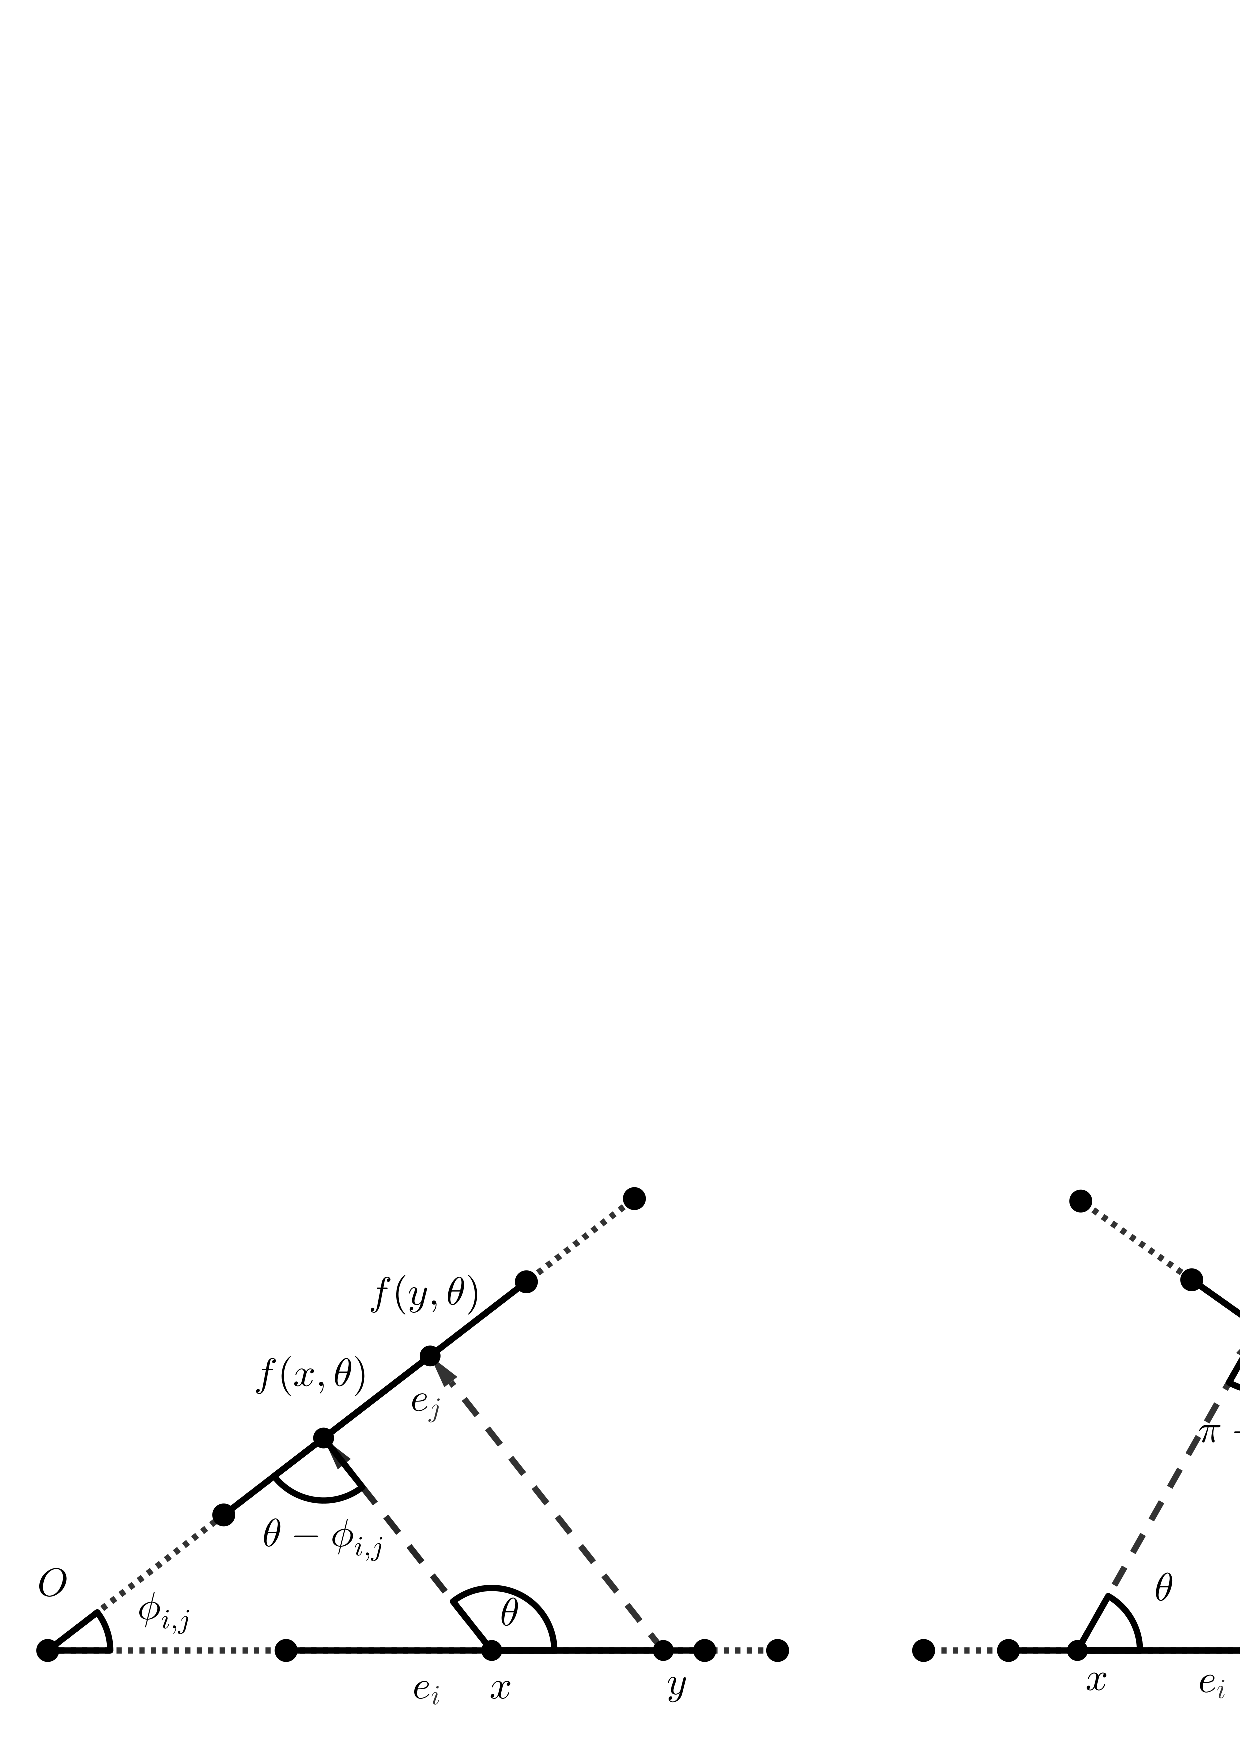
\includegraphics[width=0.9\linewidth]{../img/contraction_map_cond.pdf}
\end{center}

\vspace{-2em}

$$
c(\theta, i,j)
= \frac{|f(x, \theta) - f(y, \theta)|}{|x-y|}
= \frac{\sin(\theta)}{\sin(\theta) \pm \phi_{i,j}}
$$

Nice properties:

\begin{itemize}\compresslist
\item $c(\theta,i,j) < 1$ indicates shrinking set.
\item Given $\theta$ and a pair of segments, holds for everywhere along segments.
\item Composition: transition from edge $i$ to $j$ to $k$ has contraction
coefficient $c(\theta, i, j) * c(\theta, j, k)$.
\end{itemize}
}


%----------------------------------------------------------------------------------------
%	LIMIT CYCLES IN CONVEX POLYGONS
%----------------------------------------------------------------------------------------

\headerbox{Tasks and Behaviors}{name=convex,column=1,bottomaligned=question,below=map,span=1}{

General approach: discrete search in visibility graph while checking constraints
and criteria.

\begin{itemize}\compresslist
\item {\bf Navigation:} Strategy gets robot from start to goal states (points
on boundary).
\item {\bf Patrolling:} Repeatedly visit a set of target states (possibly in specific
order).
\item {\bf Criteria:} Fewest bounces, max-min action sets, maximally contracting
paths.
\end{itemize}


}

%----------------------------------------------------------------------------------------
%	NONCONVEXITY
%----------------------------------------------------------------------------------------

\headerbox{Example}{name=nonconvex,column=2,row=0,span=1}{ 
\begin{center}
\includegraphics[width=0.7\linewidth]{../img/cycle1.pdf}
\end{center}
}

%----------------------------------------------------------------------------------------
%	RESULTS 2
%----------------------------------------------------------------------------------------
\headerbox{Critical Angles}{name=chaos,column=2,span=1,below=nonconvex}{ 

\begin{itemize}\compresslist

\item $c(\theta, i, j)$ easy to check for a single $\theta$...
\item How to reason about sets of actions $\tilde{\theta} \subset [0, \pi]$?
\item As $\theta$ sweeps, visible edges will shrink and grow, and occasionally appear
and disappear. Contraction property may also change.
\item This information can be pre-computed and stored in the roadmap.

\end{itemize}

}


%----------------------------------------------------------------------------------------
%	FORMAL METHODS
%----------------------------------------------------------------------------------------

\headerbox{Language Design}{name=fm,column=2,span=1,below=chaos}{

\begin{itemize}\compresslist

\item Want user to specify spatial tasks and behavioral constraints.
\item Tool should give feedback on feasibility and dynamical structure of
resulting behavior.
\item Visual, interactive interface?

\end{itemize}

}




%----------------------------------------------------------------------------------------
%	CONCLUSIONS
%----------------------------------------------------------------------------------------



%----------------------------------------------------------------------------------------
%----------------------------------------------------------------------------------------
%	ACKNOWLEDGMENTS
%----------------------------------------------------------------------------------------

\headerbox{Acknowledgments}{name=acknowledgments,column=2,span=1,bottomaligned=convex,
below=fm}{
\footnotesize{
\textbf{Funding}: NSF grants 1035345 and 1328018, and CONACyT
post-doctoral fellowship 277028 \\
%\vspace{-3.5em}
}
\printbibliography[heading=none]


}
%----------------------------------------------------------------------------------------
%	REFERENCES
%----------------------------------------------------------------------------------------

%\headerbox{References}{name=references,column=1,above=bottom}{
%
%\tiny{
%
%
%1. Woese, C., et al. PNAS, 4576–4579 (1990).\\
%2. Zomer, A., et al. PLoS ONE 7, e43012 (2012).\\
%3. Solaimanpour, S., et al. PLOS ONE 10, e0126070 (2015).\\
%4. Makarova, K., , et al. Life 5, 818–840 (2015).
%
%
%}}
%
%----------------------------------------------------------------------------------------
%	FUTURE RESEARCH
%----------------------------------------------------------------------------------------
%
%\headerbox{Future Research}{name=futureresearch,column=1,span=2,aligned=references,above=bottom}{ % This block is as tall as the references block
%
%\begin{multicols}{2}
%Integer sed lectus vel mauris euismod suscipit. Praesent a est a est ultricies pellentesque. Donec tincidunt, nunc in feugiat varius, lectus lectus auctor lorem, egestas molestie risus erat ut nibh.
%
%Maecenas viverra ligula a risus blandit vel tincidunt est adipiscing. Suspendisse mollis iaculis sem, in \emph{imperdiet} orci porta vitae. Quisque id dui sed ante sollicitudin sagittis.
%\end{multicols}
%}
%




\end{poster}

\end{document}
